\section{樹狀數組}
    樹狀數組又稱為BIT,是個快速動態求取區間和的助手。

    \subsection{回顧}
    還記得前綴和嗎,他也是用來求區間和的,但你應該會發現,若當中有一個值需要被修改,那整列都會被動到,
    因此複雜度就會增加。

    以下是一個比較表,可以讓你了解BIT的強大之處。

    \begin{center}
    \begin{tabular}[h]{c|c|c}
        資料結構 & 查詢區間和 & 單點修改值 \\
        \hline
        純陣列 & $O(n)$ & $O(1)$ \\
        前綴和 & $O(1)$ & $O(n)$ \\
        BIT & $O(\log(n))$ & $O(\log(n))$ \\
    \end{tabular}
    \end{center}
    
    \subsection{用途與概念}
    BIT用於在快速求取區間和的同時,又能保證快速修改。
    感覺像是陣列與前綴和的優點結合下的產物,不過其複雜程度也是三者之中最高的。
    示意圖中數字代表它儲存的區間。

    \begin{figure}
        \centering
        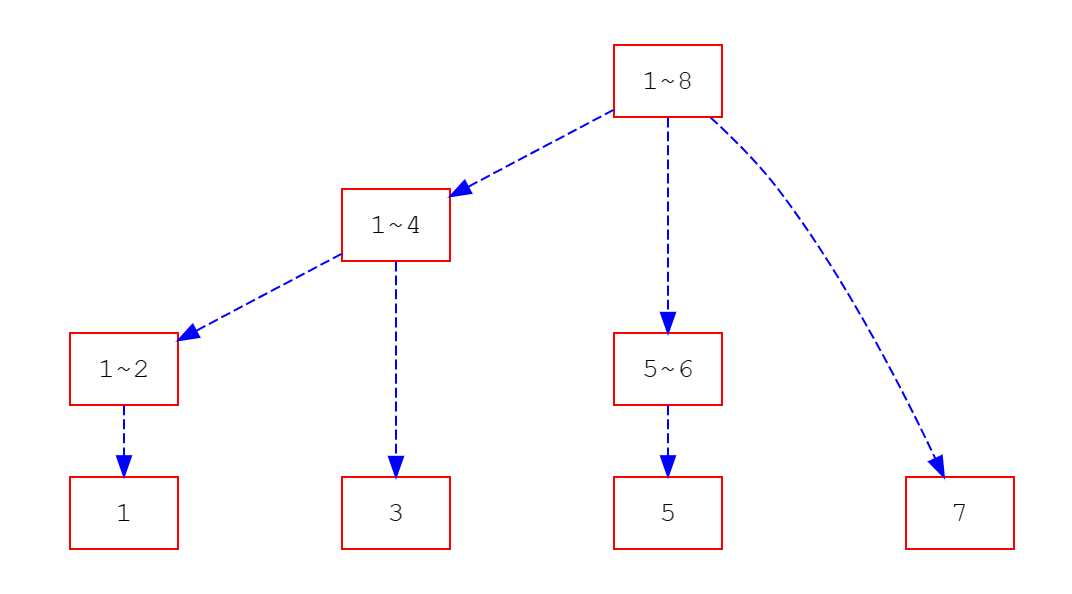
\includegraphics[width=\textwidth]{../Images/BIT.png}
        \caption{BIT 示意圖}
    \end{figure}

    如果想要知道\verb|1-5|的和,可以查詢\verb|1-4+5|。以下為查詢所需區間表。

    \begin{center}
    \begin{tabular}{|c|c|c|c|c|c|c|c|}
        \hline
        1 & 1--2 & 1--3 & 1--4 & 1--5 & 1--6 & 1--7 & 1--8 \\
        \hline
        1 & 1--2 & 1--2 \& 3 & 1--4 & 1--4 \& 5 & 1--4 \& 5--6 & 1--4 \& 5--6 \& 7 & 1--8 \\
        \hline
    \end{tabular}
    \end{center}

    可以發現,在元素數量為$8$時,最多會需要查詢$3$個區間就可以得到\verb|1-n|的值,接著就像前綴和那樣,用\verb|1~R - 1~(L-1)|就可以求出所有區間的和了。

    \subsection{實作}
    BIT一般都是用陣列實作,用區間最大值作為存放位置(例如\verb|1-4|放在\verb|4|)。那搜尋與修改呢?
    這部分就比較複雜了,需要了解一些二進位制,如果你已經理解二進位制了,那就繼續往下看吧。

    \textbf{lowbit}

    lowbit是在二進位下右邊看過來最前面的1,例如:6(000110)就是2(000010)

    \textbf{查詢}

    可以發現,$x$重複$-lowbit(x)$會變成0,且途中會經過所有需要的區間。以7為例。

    $$7(000111) \to 6(000110) \to 4(000100 \to 0(000000))$$
    
    只要將所有經過的區間加在一起,就可以得到區間和了。這也呼應為何他查尋的複雜度為$O(log(n))$,因為$n$最多只會有$log(n)$個$bit$。

    \textbf{修改}

    修改也有些相似,變成$x$加上$lowbit(x)$,就會將上面有包含到他的區間也都更新到。以$3$為例。

    $$3(000011) \to 4(000100) \to 8(001000)$$

    因為每一次都會進位,所以這樣最多也是$O(log(n))$。也可以發現$lowbit$的重要性。

    \textbf{程式碼}

\begin{lstlisting}[caption=BIT]
#define lowbit(x) (x&-x)
// 與 int lowbit(int x){ return x&-x;}
// 用define或函式雖然不會讓你的程式碼寫起來比較快,但可以使其較易於理解。

using ll=long long;

ll bt[200010];
ll a[200010];

// build 函式是透過逐個更新陣列的所有元素來建構BIT
void build(int n){
    for(int i=1;i<=n;++i)
        for(int x=i;x<200005;x+=lowbit(x))
            bt[x]+=a[i];
}

// 單點加值
void add(int x,int k){
    a[x]+=k;
    for(int i=x;i<=200005;i+=lowbit(i))
        bt[i]+=k;
}

// 由單點加值衍生出來的單點修改
void modify(int x,int k){
    add(x,k-a[i]);
}

// 搜尋1~x的區間和
ll find_sum(int x){
    ll ret=0;
    for(int i=x;i>0;i-=lowbit(i))
        ret+=bt[i];
    return ret;
}

// 用計算(1~r) - (1~(l-1))算出所有區間的區間和
ll query(int l,int r){
    return find_sum(r)-find_sum(l-1);
}
\end{lstlisting}

    \subsection{範例與練習}
    \problem ZJ d796 區域調查(POJ.1195 Mobile phones 改編)

    \textbf{題目敘述}

    給一個矩陣 $T(1,1), T(1,2),.... T(N,M)$,求 $T(x1,y1)$  到 $T(x2,y2)$ 的總和 或者是修改 $T(x1,y1)$ 的值。

    \textbf{輸入說明}

    每組輸入的第一行會有兩個正整數 $N \; Q$ $( 1 \le N \le 250,  Q \le 5 \times 10^5)$

    接下來會有 $N$ 行,每行上會有 $N$ 個元素 $M$ $( 0 \le M \le 32767 )$

    接下來會有 $Q$ 行,倘若第一個數字為$1$,則接下來會有四個數字

    $x_1 , y_1 , x_2 , y_2, 1 \; x_1 , y_1 , x_2 , y_2 \le 250$

    請輸出元素 $S={( x , y ) \; | \; x_1 \le x \le x_2, y_1 \le y \le y_2 }$符合的所有元素總和

    倘若第一個數字為$2$,則接下來會有三個數字

    $x1 , y1 , V, 1 \le x_1 , y_1 \le 250 , 0 \le V \le 32767$

    請修改 ( x1 , y1 )= V ,此行不必輸出。

    \textbf{輸出說明}

    若為調查,則輸出區域中的元素總和,若為修改,則不必輸出。

    \textbf{範例測試}

    \begin{tabular}{|m{7cm}|m{7cm}|}
        \hline
        範例輸入 1 & 範例輸出 1 \\
        \hline
        \verb|5 10|      & \verb|2| \\
        \verb|3 2 2 3 7| & \verb|42| \\
        \verb|4 4 0 3 8| & \verb|15| \\
        \verb|2 4 7 2 3| & \verb|13| \\
        \verb|5 9 6 1 4| & \verb|24| \\
        \verb|7 1 7 1 1| & \verb|33| \\
        \verb|2 2 2 1| & \\
        \verb|1 5 4 5 5| & \\
        \verb|2 2 1 7| & \\
        \verb|1 3 2 1 5| & \\
        \verb|1 2 5 4 5| & \\
        \verb|1 1 2 2 1| & \\
        \verb|2 2 2 7| & \\
        \verb|2 4 5 5| & \\
        \verb|1 3 3 4 5| & \\
        \verb|1 4 3 2 2| & \\
        \hline
    \end{tabular}

    \begin{tip}
        BIT同樣可以做成二維。
    \end{tip}

    \problem ZJ d847 98學年度中投區資訊學科能力競賽 2D rank finding problem

    \textbf{題目敘述}

    二度空間上的排名計算問題(2D rank finding problem):
    給定二度平面空間$(2D)$上的點$A = (a1,a2)$與點$B = (b1,b2)$,
    其大小關係定義為若$A > B$若且唯若 $a1> b1$ 且 $a2 > b2$,亦即A點在B點的右上方。
    值得注意的是,並非任意兩點均可以決定大小關係,如下圖中的點A與點E,點D與點E等,無法決定這兩點的大小關係故為無法比較$(incomparable)$。
    給定N個點$(x1,y1), (x2,y2), \cdots, (xn,yn)$,
    定義某一個點的排名$(rank)$ 為所給的點集合中,比該點小的點的個數。

    設計一個程式,從檔案讀取點的名稱與座標,計算出在所給定的集合中,所有點的排名值。

    \textbf{輸入說明}

    有多組測試資料

    每組的第一行有一個數字$N \; ( 1 \le N \le 10000 )$

    接下來會有$N$行,每行上會有兩個數字  $x, \; y \; ( 1 \le x , y \le 1000 )$

    \textbf{輸出說明}

    請按照輸入的順序,求出對於 $( x , y )$ 有多少個點 $( a , b )$

    在它的左下方 $a < x , b < y$

    \textbf{範例測試}

    \begin{tabular}{|m{7cm}|m{7cm}|}
        \hline
        範例輸入 1 & 範例輸出 1 \\
        \hline
        \verb|5|      & \verb|2| \\
        \verb|961 404| & \verb|1| \\
        \verb|640 145| & \verb|4| \\
        \verb|983 888| & \verb|0| \\
        \verb|539 71| & \verb|0| \\
        \verb|437 532| & \\
        \hline
    \end{tabular}

    \problem 低地距離(2020年10月APCS)

    \textbf{題目敘述}

    輸入一個長度為 $2n$ 的陣列,其中 $1 - n$ 的每個數字都剛好各 $2$ 次。

    $i$ 的低窪值的定義是兩個數值為 $i$ 的位置中間,有幾個小於 $i$ 的的數字。

    以 $[3, 1, 2, 1, 3, 2]$ 為例,$1$的低窪值為 $0, 2$ 的低窪值值為 $1, 3$ 的低窪值為 $3$。

    請對於每個 $1 - n$ 的數字都求其低窪值(兩個相同的數字之間有幾個數字比它小),輸出低窪值的總和,答案可能會超過 $C++$ $int$ 的上限。

    \textbf{輸入說明}

    第一行有一個正整數 $n, \; n \le 10^5$

    第二行有 $2n$ 個正整數,以空格分隔,
    保證 $1 - n$ 每個數字都恰好出現兩次。


    \textbf{輸出說明}

    輸出 $1 - n$ 每個數字的低窪值總和。

    \textbf{範例測試}

    \begin{tabular}{|m{7cm}|m{7cm}|}
        \hline
        範例輸入 1 & 範例輸出 1 \\
        \hline
        \verb|3|      & \verb|4| \\
        \verb|3 1 2 1 3 2| & \\
        \hline
    \end{tabular}